\section{Two-pass Event Detection Model} \label{sec:algorithm}
This section describes the modeling approach and the implementation details of our event detection algorithm.
We begin by presenting concepts of graph wavelets and their properties in Section~\ref{sec:graph_wavelet}.
Section~\ref{sec:abnormalgroupdetection} discusses applications of graph wavelets in group anomaly detection. Lastly, Section~\ref{sec:event_detection} describes the group absenteeism based two-pass event detection algorithm in detail.
\subsection{Graph Wavelets}
\label{sec:graph_wavelet}
Classic wavelet is called mathematical microscope since it is capable of showing signal abnormality with different scales.
In the case of complex networks, graph wavelets render the graph with good localization properties both in frequency and vertex (i.e. spatial) domains. Their scaling property allows us to zoom in/out of the underlying structure of the graph.

%It is useful to analyze $f$ by taking into account the intrinsic geometric structure of the graph $\mathbf{G}$. In order to identify and exploit structure of  $f\in \mathbb{R}^N$, the spectral graph $\sigma({\mathcal{L}}):=\{\chi_l\}_{l=0}^{N-1}$ can be used as a dictionary of atoms~\cite{shuman_ACHA_2013}. Thus, $f$ can be decomposed as a linear combination of $\{\chi_l\}_{l=0}^{N-1}$ as
%\begin{equation}
%\label{eq:graph_fourier}
%f(n)= \sum\limits_{l=0}^{N-1}\hat{f}(l)\chi_l(n)
%\end{equation}
%, where
%\begin{equation}
%\label{eq:graph_fourier1}
%\hat{f}(l):= \sum\limits_{n=0}^{N-1}\chi^*_l(n)f(n)
%\end{equation}
%$\chi_l$ is called the Fourier frequency of $f(n)$ based on the graph $\mathbf{G}$, and $\hat{f}(l)$ is the corresponding Fourier coefficient.
%Equation~\ref{eq:graph_fourier1} and Equation~\ref{eq:graph_fourier} are called Fourier transform and inverse Fourier transform, respectively.
%Equation~\ref{eq:graph_fourier1} gives a clear representation of the Fourier components in $f(n)$.

Recall from Equation~\ref{eq:graphFourier1}, the anomaly pattern $\hat{f}(l)$ presents the anomaly components of $f$ based on $\mathbf{G}$ from the whole graph prospective. However, information concerning the vertex-location can not be identified from the Fourier transform. To address this issue, Hammond et al.~\cite{hammond2011wavelets} proposed constructing wavelet transforms of functions over the vertices using weighted graphs, described in the following steps:

\begin{enumerate}
\item Define a continuous generating kernel functions $g(x)$ on $\mathbb{R}^+$;
\item Then, select a central vertex $v_a \in {V}$ and scale $s$, set the frequency coefficients as $g(s\lambda_l)\chi^*_l(a)$ for each frequency component $\chi_l$;
\item Finally, sum up all those frequency components $\chi_l$.
\end{enumerate}
In this way, the graph wavelet at central vertex $v_a$ is constructed as:
\begin{equation}
\label{eq:graphwaveletdefinition}
\psi_{s,a}(n) = \sum\limits_{l=0}^{N-1}g(s\lambda_l)\chi_l^*(a)\chi_l(n)
\end{equation}
After setting up the graph wavelet, the wavelet coefficients for $f$ can be defined as
\begin{equation}
\label{eq:graph_graphwavelet}
W_f(s,a)=<\psi_{s,a}, f>=\sum\limits_{l=0}^{N-1}g(s\lambda_l)\hat{f}(a)\chi_l(n)
\end{equation}
%\paragraph{\textbf{Properties}}

Similar to classical wavelets, graph wavelets provide following three properties, which are presented in detail in~\cite{hammond2011wavelets}.
 \begin{enumerate}
 \item \textbf{Reconstruction.}
 When generating the kernel function $g(x)$ satisfies the admissibility condition and $g(0)=0$,  $f(n)$ can be reconstructed by the wavelet coefficients.
\item \textbf{Discretization and Wavelet Frames} For practical applications, scale $s$ of graph wavelet $\psi_{s,a}$ should be sampled with a finite number of scales. Given a real valued function $h(x)$, satisfying
\begin{equation}
\hat{h}(\omega) = \sqrt{\int_\omega^\infty\frac{|\hat{g}(\omega')|^2}{\omega'}d{\omega'} }
\end{equation}
, where $\hat{g}$ and $\hat{h}$ are the classical Fourier transform of $g(x)$ and $h(x)$, the scaling function $\phi_{a}(n)$ can be generated as:
\begin{equation}
\label{eq:graphscaledefinition}
\phi_{a}(n) = \sum\limits_{l=0}^{N-1}h(\lambda_l)\chi_l^*(a)\chi_l(n)
\end{equation}
Accordingly, the scaling coefficients are defined as
\begin{equation}
S_f(a)=<\phi_a,f>
\end{equation}
Using scale set $\Theta:=\{s_j\}_{j=1}^J$, the discretized graph wavelet set $\{\psi_{s_j,a}\}_{j=1}^{J}$ $_{a=0}^{N-1}$, and scaling function set $\{\phi_a\}_{a=0}^{N-1}$ constitute a frame~\cite{hammond2011wavelets}.
So there will be $NJ$ wavelet coefficients in the frame.
According to frame theory~\cite{daubechies1992ten}, $f\in \mathbb{R}^N$ can be reconstructed by a limited number of scaling and graph wavelet coefficients. A detailed algorithm and treatment concerning the choice of $\Theta$ can be found in~\cite{hammond2011wavelets}.


\begin{figure}[t]
	\centering
	\subfigure[]{
		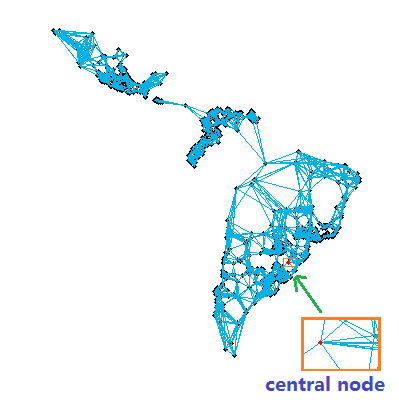
\includegraphics[height=1.6in] {figures/All-0.png}
		\label{fig:brazil1}
	}
	\subfigure[]{
		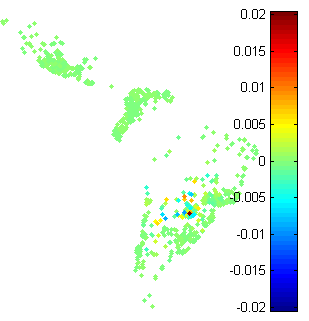
\includegraphics[height=1.6in] {figures/All-08.png}
		\label{fig:brazil2}
	}
		\subfigure[]{
		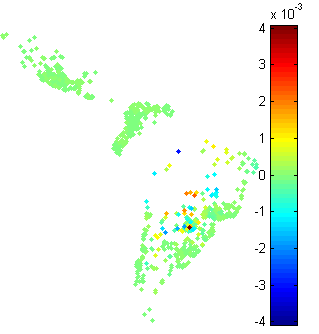
\includegraphics[height=1.6in] {figures/All-18.png}
		\label{fig:brazil3}
	}
	\subfigure[]{
		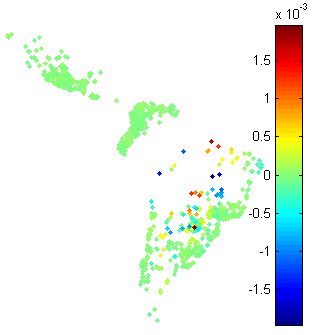
\includegraphics[height=1.6in] {figures/All-26.png}
		\label{fig:brazil4}
	}
    \subfigure[]{
		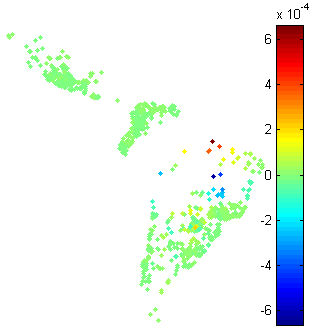
\includegraphics[height=1.6in] {figures/All-80.png}
		\label{fig:brazil5}
	}
	\subfigure[]{
		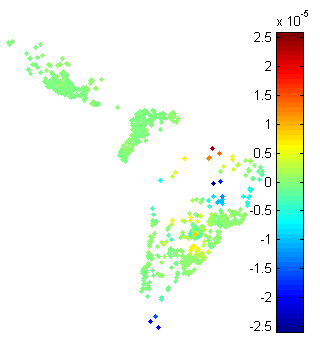
\includegraphics[height=1.6in] {figures/All-400.png}
		\label{fig:brazil6}
	}
	\caption{Spectral graph wavelet on South America. (a) vertex at which wavelets are centered in red dot. (b)-(f) wavelets, scales at 0.8, 1.8, 2.6, 8, and 40 respectively.}
	\label{fig:example2}
\end{figure}


\item \textbf{Localization in vertex domains}. Given a central vertex $v_a$ and its graph wavelet $\psi_{s,a}$, suppose the kernel function $g$ is $K+1$ times continuously differentiable, satisfying $g^{(r)}=0$ for all $r<K$ and $g^{(K)}=C\neq 0$. If there is $s'>0$ such that $|g^{(K+1)}(\lambda)|\leq B$ for all $\lambda \in [0, s'\lambda_{max}]$, let $v_n$ be a vertex of $\mathbf{G}$ such that $d_G(n,a)>K$, then there exist constants $D$ and $s''$, such that
\begin{equation}
\label{equ:waveletbound}
\frac{\psi_{s,a}(n)}{||\psi_{s,a}||}\leq Ds
\end{equation} for all $s<\min(s',s'')$.
$d_G(n,a)$ is the geodesic or shortest path distance, which is the minimum number of edges in any path that connect vertices $v_n$ and $v_a$~\cite{hammond2011wavelets}. 


Equation~\ref{equ:waveletbound} shows for any vertex $v_n$ that is far away from center vertex $v_a$ ($d_G(n,a)>K$), its wavelet value $\psi_{s,a}(n)$ is upper bounded by $Ds$. In other words, for vertex $v_n$ which is far away form vertex $v_a$, its wavelet value is linearly attenuated by scale $s$. When the scale $s$ is small, their wavelet coefficients will be vanished quickly. As shown in Figure~\ref{fig:example2}, when the scale $s$ is small, $\psi_{s,a}$ only assign weights to a small portion of vertices. As scale $s$ increases, more vertices are selected.

\end{enumerate}

\subsection{Group Anomaly Detection}
\label{sec:abnormalgroupdetection}
Recall that in Equation~\ref{eq:graphwaveletdefinition}, $||\psi_{s,a}||$ depends on scale $s$ because of the kernel function $g$. Thus for fair comparison we normalize the graph wavelet coefficient as:
\begin{equation}
\label{eq:graphwavelet}
W'_f(s,a)=<{\psi'_{s,a}}, f>=<\frac{\psi_{s,a}}{||\psi_{s,a}||}, f>
\end{equation}$W'_f(s,a)$ represents the topological distribution of $f(n)$. And for $\psi_{s,a}$ its kernel vertices denoted by $\mathcal{K}(\psi_{s,a})$, defines a set of vertices such that $d_G(n,a)\leq K$ and $0\leq\psi_{s,a}(n)$. The other vertices are called as marginal vertices. When $f$ has a uniformly large positive/negative values on the kernel vertices, $W'_f(s,a)$ is going to be a large positive/negative value as well.
Otherwise, $|W'_f(s,a)|$ will be greatly attenuated.
%Thus, large $|W'_f(s,a)|$ means a uniform distribution of $f(n)$ around vertex $v_a$ with a scale of $s$.
These weights are linearly controlled by scale $s$.
According to Equation~\ref{equ:waveletbound}, when $s$ is small, the weights of the marginal vertices are severely attenuated, and hence the weights of the kernel vertices are enhanced since $\psi_{s,a}$ is normalized.
Essentially, $W'_f(s,a)$ is equivalent to the sum of $f$ with large weights on kernel vertices, and small weights on marginal vertices.
%, and can also be treated as a similarity between $f$ and $\psi'_{s,a}$.
When $f$ is of uniformly large negative/positive value on kernel vertices, then $W'_f(s,a)$ will be a large negative/positive value with scale $s$.
We call the wavelets with minimal and maximal $W'_f(s,a)$ absenteeism wavelet and burst wavelet, respectively.


The localization property of graph wavelet makes it appropriate for group anomaly detection since it automatically identifies the kernel vertices from $V$.  These kernel vertices form a compact subset since each one of them is close to the same center vertex $v_a$. Thus, under this definition of compactness in graph wavelet, the problem of Equation~\ref{eq: problem} can then be converted to the following problem:
\emph{given a graph and \textit{absenteeism score} vector, $\mathbf{G}(V,E,W;f^t)$ at time interval $t$, select a graph wavelet $\psi_{s,a}$ and its kernel vertices $\Sigma$, such that}
\begin{equation}
 \label{eq: problem_wavelet}
    \psi_{s,a}=\underset{s_j\in \Theta, v_n\in V}{\arg\min} {W'_f(s_j,n)}
\end{equation}, and
\begin{equation}
 \label{eq: problem_wavelet_3}
    \Sigma=\mathcal{K}(\psi_{s,a})
\end{equation}
As Equation~\ref{eq: problem_wavelet} avoids the compactness constrain condition, thus its complexity is greatly reduced.

Figure~\ref{fig:graphwaveletscale} shows two graph wavelets centered on the same vertex $v_a$, but with two different scales, $\psi_{s_1,a}$ and $\psi_{s_2, a}$, where $s_1<s_2$. The length of the black bar on each vertex denotes its graph wavelet value. The highlighted areas denote the kernel vertices with larger graph wavelet values.
Figure~\ref{fig:scale3} is $f$'s distribution along each vertex, whose value is denoted as the vertical bar. As we can see, with the graph wavelet pattern of $\psi_{s_2,a}$, $f$ shows a larger value on most of the kernel vertices, and $W'_f(s_2,a)$ a large value as well. That also means $\psi_{s_2,a}$ optimally partitions the set $V$ into two distinct groups - kernel and marginal vertices. As shown in Figure~\ref{fig:scale4}, $W'_f(s_3,a)$ is where the absenteeism is most significant, and $W'_f(s_2,a)$ is  where bursty behavior is observed.

\begin{figure*}[t]
	\centering
	\subfigure[wavelet $\psi_{s_1,a}$]{
		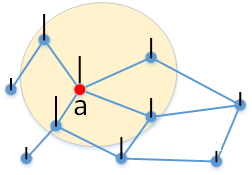
\includegraphics[width=1.4in, height=1.2in] {figures/wavelet1.png}
		\label{fig:scale1}
	}
	\subfigure[wavelet $\psi_{s_2,a}$]{
		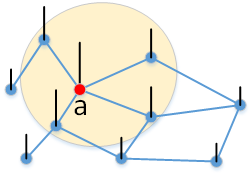
\includegraphics[width=1.4in, height=1.2in] {figures/wavelet2.png}
		\label{fig:scale2}
	}
\subfigure[$f(n)$ vs vertices]{
		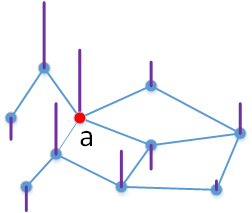
\includegraphics[width=1.4in, height=1.2in] {figures/wavelet3.png}
		\label{fig:scale3}
	}
\subfigure[$W'_f(s,a)$ vs scale $s$]{
		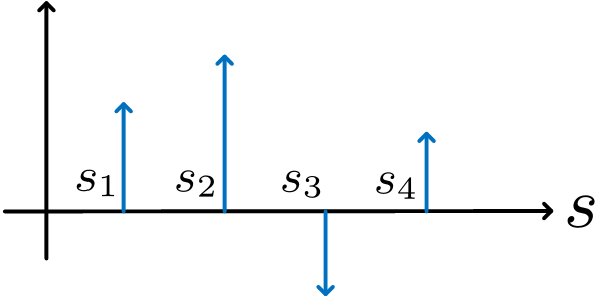
\includegraphics[width=1.7in, height=1.2in] {figures/wavelet4.png}
		\label{fig:scale4}
	}
\vspace{-2mm}
	\caption{Using graph wavelets for abnormal group identification.}
	\label{fig:graphwaveletscale}
\end{figure*}


\paragraph{\textbf{Remarks}}
\begin{enumerate}
\item As graph wavelet and scaling functions form a frame, the function $f$ can be reconstructed by their coefficients.
As long as the scale level $J$ is high enough, $f$ can be well decomposed into the frame basis. Thus, using graph wavelets to exploit structure of functions defined on graphs is much more reasonable.

\item Graph wavelet transforms select vertices that are close to the central vertex $v_a$, and attenuate the impact of other marginal vertices that are far away from $v_a$.
Unlike other conventional methods,  $\psi_{s,a}$ is automatically scalable, and maintains the graph's topological information.

\item The graph wavelet does not introduce any objective functions and constraints. In addition, the scale $\{s_j\}_{j=1}^J$ set is numerically small, and once the eigenvalues and eigenvectors of $\mathbf{G}$ are known, the computation complexity of graph wavelet coefficients is $O(NJ)$, which makes is easily adaptable to wide variety of application scenarios.
\end{enumerate}

\subsection{Group Absenteeism Based Event Detection}
\label{sec:event_detection}
This section proposes a novel two-pass absenteeism based event detection algorithm. The underlying rationale of this algorithm is based on the following concepts.
\begin{enumerate}
\item As discussed in section~\ref{sec:graph_wavelet}, distribution of $f$ can be well reconstructed by the $J$ scaling and $NJ$ wavelet coefficients. Each of those normalized wavelet coefficients $W'_f(s,a)$ represents a distribution pattern of $f$ on $\mathbf{G}$.
It is equivalent to saying that $\psi_{s,a}$ represents a special distribution pattern, which shares a large and uniform value around the central vertex with scale $s$.
\item When a significant event occurs, preceded by group absenteeism behavior in social networks, such as a severe earthquake or a massive protest, it is likely to be succeeded by a spike or burst in online user activity.
With this observation, we can represent an absenteeism behavioral pattern as $\psi_{s_l,a_l}$ at time $l$ centering at vertex $v_{a_l}$, and a burst related pattern as $\psi_{s_{\tau,a_\tau}}$ at time $\tau$ centering at vertex $v_{a_\tau}$. We assume the burst pattern happens within the time window size of $L$ after absenteeism pattern is identified. Further, a notion of response time can represented using the time difference $t_{rsp}=\tau-l$.
\item Both absenteeism and burst signal must show a strong correlation, especially if they occur in close proximity spatially and temporally.
%For instance, taking the power-cut-off for instance, usually only people who live in the affected area will ``yield at " this event a lot because it brings inconvenience to their life. However, people who live outside of the affected areas would hardly mention this event. Thus, to measure the correlation between absenteeism pattern and burst pattern is proposed as:
\begin{equation}
\label{eq:eventsimilarity}
\rho(\psi_{s_l,a_1}, \psi_{s_\tau,a_\tau})= \frac{<\psi_{s_l,a_1}, \psi_{s_\tau,a_\tau}>}{||\psi_{s_l,a_1}||\cdot ||\psi_{s_\tau,a_\tau}||}
\end{equation}
Based on these concepts, the higher the correlation, the higher probability that burst patterns is caused by the preceding group absenteeism. When $\rho$ is above the threshold (threshold is set at 0.5), we infer that an event occurred and that it evolved on social networks into distinct phases: first group absenteeism, followed by a spike or burst in user activity.
\end{enumerate}

\begin{algorithm}[t]
\centering
\captionsetup{font=scriptsize}
\caption{Two-Pass Absenteeism Event Detection}
{\footnotesize \begin{algorithmic}[1]
\STATE {\bf Input:} graph and absenteeism score vector $\mathbf{G}(V,E,W;f^l)$ at time interval $l$, and time window size $L$.
\STATE {\bf Output:} correlation $\rho$ and response time $t_{rsp}$.	
\STATE{compute the spectral $\sigma{(\mathcal{L})}$ of graph $\mathbf{G}$};
\STATE{set the graph wavelets $\psi_{s,a}$ and scales set $\{s_j\}_{j=1}^J$};
\STATE{compute $W'_f(s_j, a)$ for all $v_n\in V$ and $s_j \in \{s_j\}_{j=1}^J$};
\STATE{detect the most absenteeism pattern $\psi_{s_l,a_l}$ of $f^l$}
	\FORALL {$\tau$ from $l+1$ to $l+L$}
        \STATE{calculate the most burst wavelet $\psi_{s_\tau,a_\tau}$ of $\mathbf{G}(V,E,W;f^{\tau})$ at time interval $\tau$;}
        \STATE{calculate correlation coefficients $\rho(\psi_{s_l,a_l},\psi_{s_\tau,a_\tau})$;}
	\ENDFOR	
\STATE{identify the maximal coefficients $\rho_{max}$ = $\argmax_{\tau}\rho(\psi_{s_l,a_l},\psi_{s_\tau,a_\tau})$;}
\RETURN $\rho_{max}$ and $t_{rsp}$.
\end{algorithmic}}
\label{algo:event_detection}
\end{algorithm}
In summary, the two-pass absenteeism event detection can be summarized as shown in Algorithm~\ref{algo:event_detection}. Because the computation of the graph spectral graph $\sigma(L)$ is a one-time computation, the two-pass algorithm has $O(NJ)$ complexity.
\vspace{-2mm}
\begin{enumerate}
\item Compute $\mathbf{G}$'s spectral graph $\sigma(L)$. Because $\sigma(L)$ is independent of the time interval, it is computed only once and can be solved by classical matrix factorization methods.
\item Set scale set $\{s_j\}_{j=1}^J$ according to algorithms in~\cite{hammond2011wavelets}, and the $NJ$ normalized graph wavelet coefficients $W'_f(s_j, a)$ at current time interval $l$.
\item Identify the most negative $W'_f(s_l, a_l)$, and determine the corresponding $\psi_{s_l,a_l}$ as the absenteeism pattern.
\item For all the time interval $\tau$ from $l+1$ to $l+L$, compute all the $W'_f(s_j, a)$, detect the most positive one and identify the corresponding graph wavelet $\psi_{s_\tau,a_\tau}$ as the burst pattern at time $\tau$, and the correlation score $\rho_{\tau}$ between absenteeism pattern $\psi_{s_l,a_l}$ and burst pattern $\psi_{s_\tau,a_\tau}$.
\item Detect the largest $\rho_{\tau}$ as $\rho_{max}$; return $\rho_{max}$ and response time $t_{rsp}$.
\end{enumerate}





%\paragraph{\textbf{Event Impact}}
%The absenteeism event impact is defined as:
%\begin{equation}
%AEI = (|W'_f(t_l,n_l;l)|+1)*|W'_f(t_\tau,n_\tau;\tau)|*\frac{t_\tau}{t_l}.
%\end{equation}
%\paragraph{\textbf{Response Time}} The absenteeism event response time is defined as:
%\begin{equation}
% t_{rsp}= \tau-l.
%\end{equation}
